\documentclass{beamer}
\usepackage[orientation=landscape,size=custom,width=16,height=10,scale=0.5,debug]{beamerposter}

% für deutsche umlaute und ut8
\usepackage[utf8]{inputenc}
\usepackage[T1]{fontenc}
\usepackage{lmodern} % moderne schriftart

\usepackage[english]{babel}

\usepackage[style=numeric,
            natbib=true,
            backend=bibtex
           ]{biblatex}

\addbibresource{references.bib}

\usepackage{graphicx}
\usepackage{booktabs}
\usepackage{hyperref}
\usepackage{listings}
\usepackage{tikz}
\usetikzlibrary{shapes,shadows,snakes,arrows,matrix,calc,er}
\usepackage{framed, color}

% color definitions
\definecolor{lightblue}{rgb}{0,0.6,1.0}
\definecolor{lightgray}{rgb}{0.4,0.4,0.4}
\definecolor{blue}{rgb}{0,0.3,0.6}
\definecolor{darkblue}{rgb}{0,0.1,0.4}
\definecolor{green}{rgb}{0,0.7,0.2}
\definecolor{darkerblue}{rgb}{0,0,0.4}

% design changes
\setbeamertemplate{footline}[frame number]
\setbeamercolor{title}{fg=darkerblue}
\setbeamercolor{author}{fg=lightgray}
\setbeamercolor{frametitle}{fg=darkerblue}
\setbeamercolor{background canvas}{bg=white}

\beamertemplatenavigationsymbolsempty

\setbeamercovered{transparent}

\usebackgroundtemplate{}

\renewcommand\sfdefault{phv}
\renewcommand\familydefault{\sfdefault}
% bold- text
%\renewcommand{\seriesdefault}{\bfdefault}

% todo macro
\newcommand{\todo}[1]{\textcolor{red}{#1}}
% hide macro
\newcommand{\hide}[1]{}


\newcommand{\G}[1]{\textcolor{green}{#1}}
\newcommand{\R}[1]{\textcolor{red}{#1}}
\newcommand{\B}[1]{\textcolor{blue}{#1}}
\newcommand{\vitem}{\vfill\item}

\setbeamertemplate{itemize item}{\color{blue}$\blacktriangleright$}
\setbeamertemplate{itemize subitem}{\color{blue}$\circ$}

\usebibitemtemplate{\insertbiblabel}
\usepackage[framemethod=tikz]{mdframed}

% add general things
\title{Title}
\author{Steve Göring}
\date{\today}

\begin{document}

\begin{frame}[plain, noframenumbering]
    \maketitle{}
\end{frame}

\frame{
    \tableofcontents
}

\section{First}
\frame{
    \frametitle{First Slide}
    \begin{center}
        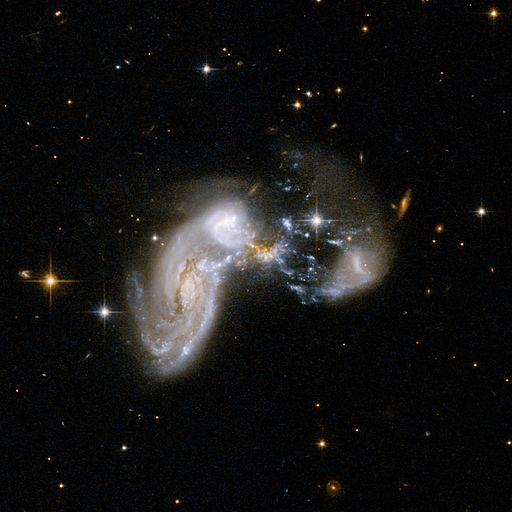
\includegraphics[width=0.5\textwidth]{figures/example1.jpg}
    \end{center}
    \begin{itemize}[<+->]
        \vitem item1
        \vitem item2
    \end{itemize}
}


\section{Table}
\begin{frame}[fragile]
    \frametitle{Frame with table}
    \begin{itemize}
        \vitem some text \cite{Berlin} \pause
    \end{itemize}
    \begin{tabular}{llrrr}
    \toprule
       \textbf{video} & \textbf{dsl [bit/s]} & \textbf{avg stalling} & \textbf{player load time} & \textbf{startup delay} \\
        \midrule
       first          & 2\,M                 & 8473                  & -620                      & 8507 \\
       (55\,s)        & 6\,M                 & -536                  & -742                      & -534 \\
                      & 25\,M                & -472                  & -749                      & -486 \\
        \midrule
       second         & 2\,M                 & 9784                  & -463                      & 8669 \\
       (121\,s)       & 6\,M                 & -322                  & -637                      & -329 \\
                      & 25\,M                & -788                  & -651                      & -785 \\
        \midrule
       third          & 2\,M                 & -800                  & -447                      & -715 \\
       (331\,s)       & 6\,M                 & -851                  & -595                      & -855 \\
                      & 25\,M                & -902                  & -651                      & -908 \\
    \bottomrule
    \end{tabular}
\end{frame}

\section{End}
\frame{
    \frametitle{Frame with table}
    Are there any questions?
}

\section{References}
\begin{frame}[t,allowframebreaks]
    \frametitle{References}
    \printbibliography
\end{frame}

\end{document}
